\documentclass{standalone}

\usepackage{tikz}
\usetikzlibrary{shapes.geometric, arrows}

\begin{document}
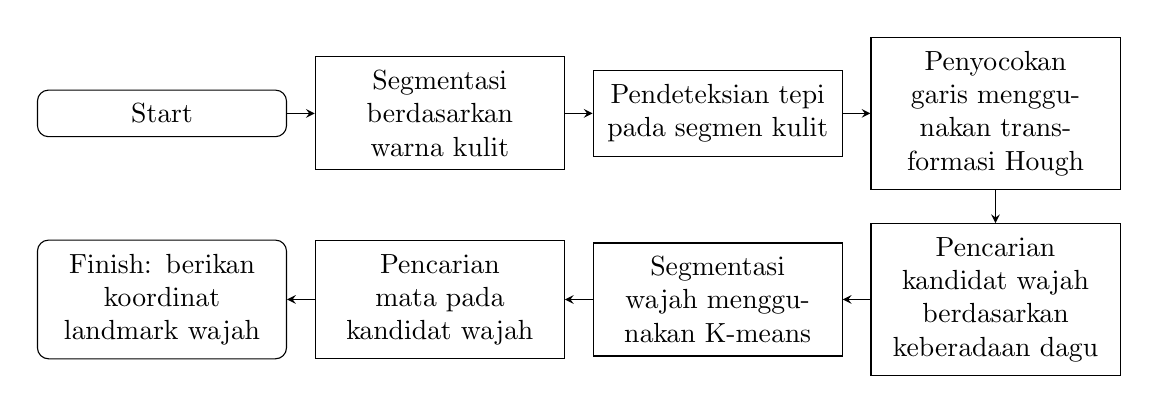
\begin{tikzpicture}[
    node distance = 2em,
    arrow/.style ={draw, thin, ->, >=stealth},
    startstop/.style = {rectangle, rounded corners, inner sep=.5em, text width=8em, text centered, draw=black},
    process/.style = {rectangle, inner sep=.5em, text width=8em, text centered, draw=black}
  ]
  \matrix[column sep=1em, row sep=1.2em]{
    \node (start) [startstop] {Start};                                   &
    \node (segkulit) [process] {
      Segmentasi berdasarkan warna kulit
    };                                   &
    \node (edgekulit) [process] {
      Pendeteksian tepi pada segmen kulit
    };                                  &
    \node (hough) [process] {Penyocokan garis menggunakan transformasi Hough};    \\
    \node (stop) [startstop] {Finish: berikan koordinat landmark wajah}; &
    \node (eyes) [process] {Pencarian mata pada kandidat wajah};         &
    \node (facesegment) [process] {Segmentasi wajah menggunakan K-means}; &
    \node (jaw) [process] {Pencarian kandidat wajah berdasarkan keberadaan dagu}; \\
  };
  \begin{scope}[every path/.style=arrow]
    \path (start) -- (segkulit);
    \path (segkulit) -- (edgekulit);
    \path (edgekulit) -- (hough);
    \path (hough) -- (jaw);
    \path (jaw) -- (facesegment);
    \path (facesegment) -- (eyes);
    \path (eyes) -- (stop);
  \end{scope}
\end{tikzpicture}
\end{document}
